\documentclass[fleqn,a4paper,11pt]{report}
\usepackage[italian]{babel}
\usepackage[margin=1in]{geometry}
\usepackage[final]{graphicx}
\usepackage{amsmath}
\usepackage{amsthm}
\usepackage{wasysym}
\usepackage{stmaryrd}
\usepackage{amsfonts}
\usepackage[utf8x]{inputenc}
\usepackage{booktabs}
\usepackage{url}
\usepackage{listings}
\lstset{mathescape,columns=fullflexible,basicstyle=\fontfamily{lmvtt}\selectfont}
\usepackage{caption} 
\setlength\abovecaptionskip{.4em}
\setlength\belowcaptionskip{.8em}
\usepackage{hyperref}
\usepackage{titlesec}
\usepackage{rotating,booktabs}
\def\MC#1{\multicolumn{1}{c}{#1}}


%\usepackage{titlesec}
%\titleformat*{\section}{\Huge\bfseries}

\usepackage{tikz}
\usetikzlibrary{calc}
\newcommand\HRule{\rule{\textwidth}{1pt}}
\newcommand\LRule{\rule{\textwidth}{.5pt}}
\newcommand\DRule{\rule{\textwidth}{.4pt}\\[\dimexpr-\baselineskip+1mm+2pt] \rule{\textwidth}{2pt}}

\usepackage{titlesec}
\titleformat{\chapter}[hang]
{\normalfont\huge\bfseries}{\chaptertitlename\ \thechapter:}{.3em}{} 

%\titlespacing*{<command>}{<left>}{<before-sep>}{<after-sep>}
\titlespacing*{\chapter}
{0pt}{5.5ex plus 1ex minus .2ex}{3.3ex plus .2ex}

\begin{document}

% begin intro
\begin{titlepage}
\begin{center}
	\begin{minipage}{6in}
  		\centering
  		\raisebox{-0.5\height}{
\includegraphics[height=80px]{img/pollo.png}}
  		\hspace*{1.6in}
  		\raisebox{-0.5\height}{
\includegraphics[height=20px]{img/logoDM.png}}
  		%\hspace*{.35in}
	\end{minipage}\\[.5cm]
% Upper part of the page
\textsc{\LARGE Universit\`a di Padova}\\[.2cm]
\textsc{\large Dipartimento di Matematica\\
			Corso di Laurea Magistrale in Informatica}\\[.3cm]
\DRule \\[.5cm]
% Title
{ \huge \bfseries Corso di Intelligenza Artificiale}\\[.4cm]
{\Large Marco Romanelli, [1106706]} \\[1cm]
{\large \today}
\HRule \\[3cm]
\end{center}
\end{titlepage}
\newpage
% end intro

%%%%%%%%%%%%
% begin document
\chapter{Introduzione}
\section{Fase iniziale}
La fase iniziale del progetto consiste in una prima analisi delle principali piattaforme che offrono servizi di \textit{Cognitive Computing}, considerando vantaggi e svantaggi di ognuna.
Data la diversificazioni di proposte all'intero di ogni piattaforma, per l'analisi e la comparazione ci siamo focalizzati sul riconoscimento di immagini.


%%%%%%%%%%%%
\section*{}
Procederemo nel seguente modo: nel Capitolo 2 verrà presentata una panoramica dei servivi presi in esame e seguirà poi nel Capitolo 3 l'analisi dettagliata per ogni servizio.
Il Capitolo 4 contiene una sintesi sulle tariffe richieste per ogni servizio.
Il Capitolo 5 riassume le conclusioni della squadra di lavoro. 
Il capitolo 6 concluderà con alcuni possibili sviluppi di questa analisi.

\section{Snippet}
In un'analisi è spesso necessario anche definire un possibile caso d'uso (obbietto) ed effettuare delle prove in relazione a tale contesto. Questo sia per approfondire l'analisi in sé e sia per poter comparare le diverse soluzioni offerte in un contesto reale (anche se limitato).

Si immagini, quindi, di dover analizzare degli scontrini fiscali con l'obbiettivo di informatizzare le informazioni contenutevi, come ad esempio il locale che ha emesso lo scontrino, le voci con i relativi prezzi, il giorno di emissione, eccetera.
Questo perché, ad esempio, un'azienda potrebbe aver bisogno di un sistema che permetta l'analisi degli scontrini per stabilire se e in che misura attribuire dei rimborsi ai propri dipendenti.

Per ogni soluzione si effettueranno alcune prove in relazione al contesto appena descritto, analizzandone pregi e difetti, tenendo ovviamente in considerazione la natura limitata delle stesse.

Tutto il codice a cui si fa riferimento si può trovare nel repository online\cite{ai-repo}.


%%%%%%%%%%%%
{\let\clearpage\relax \chapter{Cognitive Computing}}
\section{Introduzione}
% TODO

\section{Servizi disponibili}
Le maggiori piattaforme per il \textit{Cognitive Computing} sono offerte da alcune fra le maggiori aziende nell'ambito informatico e tecnologico e sono:
\begin{itemize}
\item Microsoft Cognitive Services \cite{mcs-link} (Microsoft Corporation),
\item Watson Developer Cloud \cite{ibm-link} (IBM: International Business Machines Corporation),
\item Amazon Artificial Intelligence \cite{amazon-link} (Amazon.com, Inc)
\item Google Cloud Platform (Google Inc.)
\end{itemize}


%%%%%%%%%%%%
{\let\clearpage\relax \chapter{Analisi dei servizi}}
%% Microsoft
\section{Microsoft Cognitive Services: Computer Vision API}
\subsection{Panoramica}
\paragraph{Prerequisiti}
\begin{itemize}
\item Credenziali per accedere al servizio (API key).
\item Input: dati grezzi (stream application/octet) o url.
\item Formati supportati: JPEG, PNG, GIF, BMP.
\item Dimensione file massima: 4 MB.
\item Dimensione immagine minima: 50x50 pixel.
\end{itemize}
%

Le API\cite{mcs-api} sono molteplici, a seconda dello scopo finale dell'analisi visiva.

\paragraph{Tagging} Le API ritornano un insieme di etichette (in formato JSON) che descrivono gli oggetti presenti nell'immagine, come oggetti, esseri viventi, azioni, paesaggi; per ogni etichetta viene anche fornito il livello di \textit{confidence} (affidabilità). I tag non sono in alcun modo organizzati fra loro e non esiste nessun tipo di ereditarietà.
Nel caso un tag sia ambiguo viene fornito in aggiunta un \textit{hint} che ne spiega il contenuto.
Al momento la sola lingua supportata è l'inglese.

\paragraph{Classificazione} L'immagine viene classificata in categorie che seguono una tassonomia con ereditarietà di tipo padre-figlio. Questa tassonomia prevede 86 categorie\footnote{\url{https://www.microsoft.com/cognitive-services/en-us/Computer-Vision-API/documentation/Category-Taxonomy}} e classifica gli elementi visivi in modo più o meno specifico.

\paragraph{Identificazione del tipo} E' possibile classificare l'immagine come in bianco o nero o a colori, se è un disegno o se è del tipo \textit{clip-art}; in quest'ultimo caso viene fornito un livello di qualità dell'immagine, compreso fra 0 e 3.

\paragraph{Riconoscimento volti} Riconosce i volti umani e restituisce la posizione (coordinate) di questi all'interno dell'immagine, come anche età e sesso della persona.

\paragraph{Contenuto personalizzato} Ideato per raffinare la tassonomia a 86 categorie utilizzando informazioni specifiche sul dominio. Attualmente è supportato solamente il riconoscimento dei volti delle persone famose.

\paragraph{Generazione di descrizioni} Genera una lista di frasi (in lingua inglese) che descrivono il contenuto dell'immagine, ordinate secondo un livello di affidabilità calcolato per ogni descrizione.

\paragraph{Estrazione colori} Identifica i colori analizzandoli in tre contesti: di sfondo, in primo piano e d'insieme; i colori sono raggruppati in 12 colori predominanti. Classifica le immagini fra in bianco e nero e a colori.

\paragraph{Riconoscimento contenuti non adatti ai minori} Riconosce materiali pornografici e contenuti osé in generale. Può essere impostato un livello per il filtro.

\paragraph{Riconoscimento del testo (OCR)} Rileva il testo presente nell'immagine e lo trasforma in un flusso di parole, ruota l'immagine se necessario per rendere il testo orizzontale e fornisce le coordinate per ogni parola. Al momento sono supportati 21 linguaggi, fra cui l'inglese, l'italiano, il francese, il tedesco e lo spagnolo.

L'accuratezza del riconoscimento dipende dalla qualità dell'immagine ed eventuali errori possono essere causati da immagini sfuocate, scrittura a mano, testo troppo piccolo, ecc.
   
\paragraph{Creazione anteprime} Un'anteprima è una rappresentazione dell'immagine in scala ridotta. L'immagine viene prima analizzata e poi ritagliata secondo la ``regione di interesse'' (ROI); il rapporto dell'immagine (\textit{aspect ratio}) può essere impostato secondo le proprie preferenze.

\subsection{Tariffe} Due tipologie di piani:
\begin{itemize}
\item Gratuito: fino a 5000 chiamate al mese, massimo 20 chiamate al minuto;
\item Standard: 0,015\$ a chiamata, fino a 10 TPS.
\end{itemize}

\subsection{Esecuzione}
Prendendo in esame il caso d'uso descritto nell'introduzione, sono state sono state individuate due tipologie di operazioni che potrebbero risolvere il problema posto: estrazioni di caratteristiche visive (e classificazione) e l'OCR.

\paragraph{Estrazione \textit{features} e classificazione} Come si vede nell'immagine ~\ref{ms-analyze}, il contenuto viene classificato come \textit{text menu} con un livello di \textit{confidence} dell'$85,5\%$.
\begin{figure}[htbp]
\begin{center}
	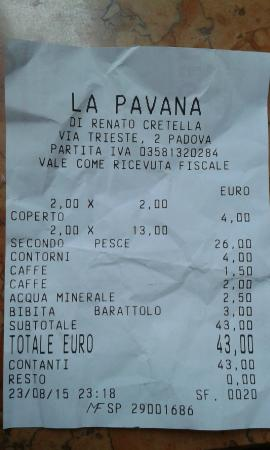
\includegraphics[height=.3\textwidth]{img/scontrino.jpg}
	 \hspace*{.5in}
	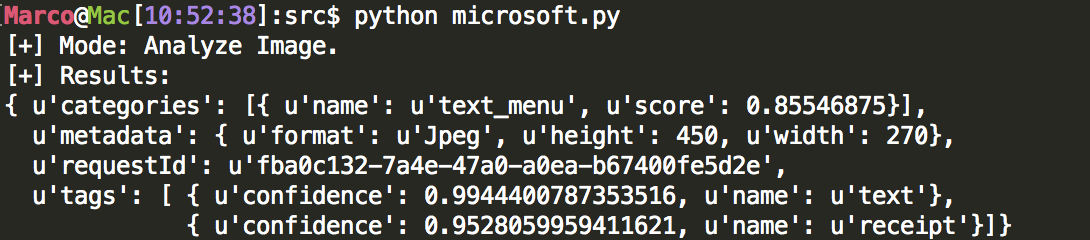
\includegraphics[height=.1\textwidth]{img/ms-analyze.png}
\caption{Estrazione delle caratteristiche.}
\label{ms-analyze}
\end{center}
\end{figure}
Vengono create anche le etichette \textit{text} e \textit{receipt}, entrambe con un alto livello di affidabilità. Quindi l'algoritmo identifica correttamente il contenuto e il significato astratto dell'immagine: è uno scontrino, o comunque una lista di elementi testuali.

Tuttavia, seppur l'analisi sia corretta, non raggiunge il nostro obbiettivo di estrarre la lista di elementi dello scontrino.

\paragraph{OCR} La seconda funziona che sembrerebbe essere adatta al nostro obbiettivo è il riconoscimento del testo. 
\begin{figure}[h!]
\begin{center}
	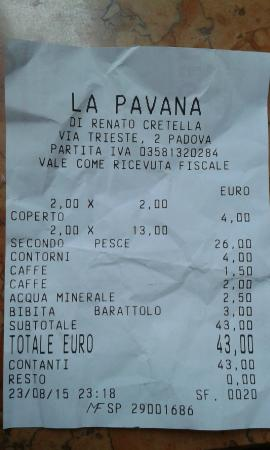
\includegraphics[height=.3\textwidth]{img/scontrino.jpg}
  	\hspace*{.5in}
	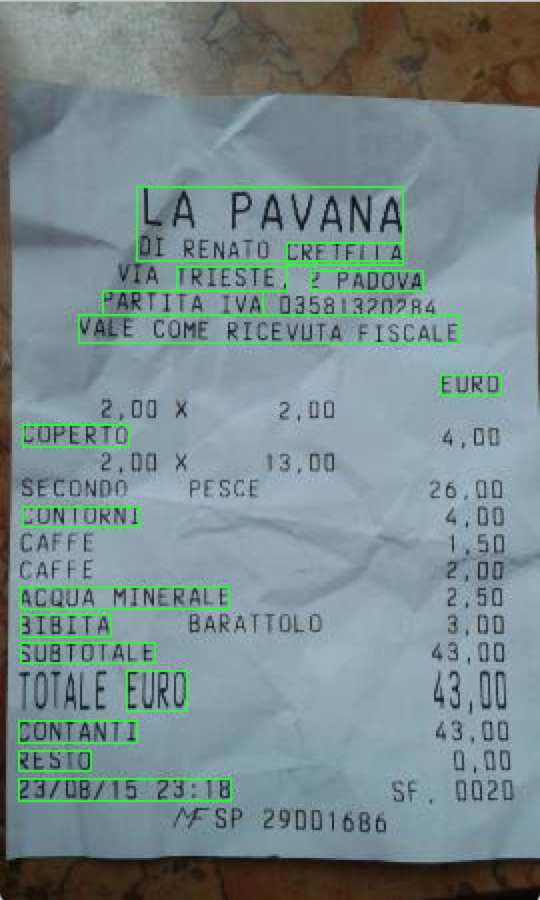
\includegraphics[height=.3\textwidth]{img/ms-ocr.png}
	  	\hspace*{.5in}
	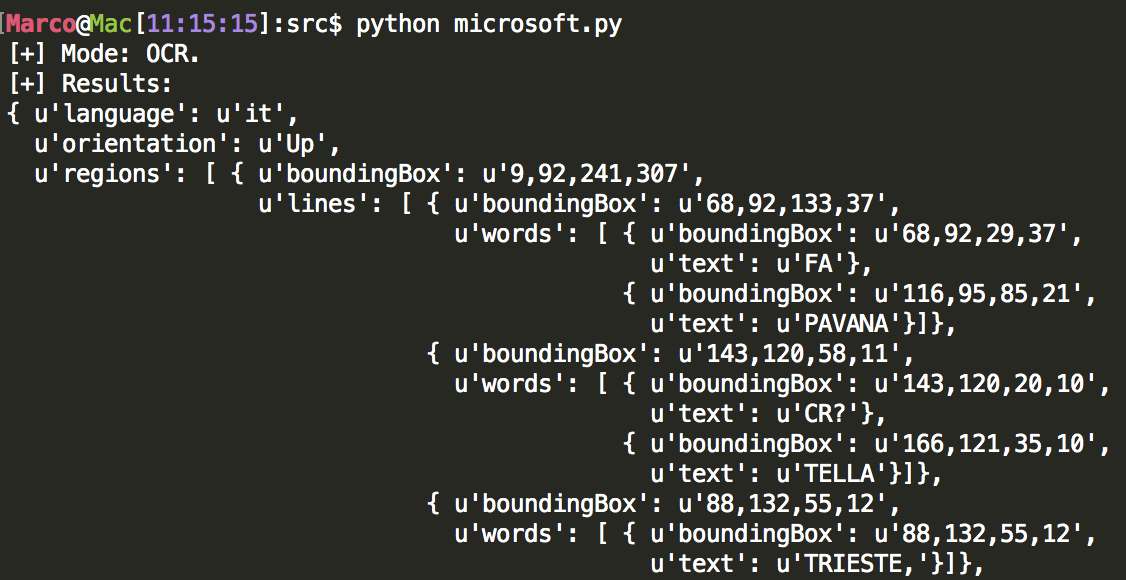
\includegraphics[height=.2\textwidth]{img/ms-ocr-2.png}
\caption{Estrazione del testo.}
\label{ms-ocr}
\end{center}
\end{figure}
Dalla figura si vede come l'algoritmo sia riuscito a rilevare molte parole (ma non tutte) ma non i numeri (i prezzi); inoltre si nota come diverse parole siano state \textit{tradotte} erroneamente, come \textsf{capERTO} invece che ``coperto'' o \textsf{COMANI} al posto di ``contanti''.


In conclusione non si ritiene il risultato sufficiente per lo scopo prefissato. 

%% Microsoft
\section{IBM Developer Cloud: Visual Recognition}
\subsection{Panoramica}
Il servizio di Visual Recognition\cite{ibm-api} utilizza tecniche e algoritmi di \textit{deep learning} per identificare scene, oggetti, visi di persone nell'immagine che viene fornita come input al servizio. Permette, inoltre, la creazione e l'addestramento di un classificatore personalizzato per l'identificazione di elementi in base alle necessità dello sviluppatore.

\paragraph{Requisiti}
\begin{itemize}
\item Credenziali per accedere al servizio (API key).
\item input: dati grezzi o URL all'immagine.
\item formati supportati: JPG, PNG.
\item dimensioni minime: 224x224 pixel (consigliate).
\end{itemize}

\paragraph{Classificazione} Per ogni immagine sottoposta a classificazione viene fornito in riposa una lista di coppie classe-punteggio per ogni classificatore selezionato. Il punteggio è compreso in un intervallo $0-1$, dove un valore maggiore indica una probabilità più alta che la classe descriva l'immagine; la soglia di default perché un valore sia ritornato da un classificatore è $0,5$.
Le classi sono organizzate in categorie e sotto-categorie dove il livello più astratto comprende categorie quali animali, persone, cibo, sport, natura, eccetera.

Le lingue sopportate\footnote{Al momento della stesura di questo documento.} nella risposta sono l'inglese, spagnolo, arabo o giapponese. 

\paragraph{Riconoscimento dei volti} Analizza i volti presenti l'immagine e ne deriva alcune informazioni, come età stimata, sesso o nome del personaggio famoso (nel caso ci sia). Anche in questo caso viene fornito un punteggio (nell'intervallo $0-1$) atto ad indicare una maggiore probabilità di correlazione.

\paragraph{Classificatore personalizzato} Permette di creare un nuovo classificatore e di addestrarlo su un dato insieme di immagini. Queste sono inviate in un file compresso e devono comprendere o due immagini d'esempio positive o una positiva e una negativa. L'insieme contente le immagini d'esempio positive serve a creare le classi che definiscono il nuovo classificatore. Il complementare definisce invece quello che il classificatore \textit{non} deve essere; le immagini d'esempio negative non devono contente i soggetti presenti nelle immagini positive.

Se, ad esempio, si volesse creare un classificatore ``frutta'' si potrebbe utilizzare un file compresso contente immagini di pere, uno contente immagini di mele e uno con immagini di banane.
Per le immagini d'esempio negative si potrebbero utilizzare immagini di verdure.

\paragraph{Collezioni} Questa funzione\footnote{Questa funzione è ancora in fase BETA} permette di creare una nuova collezione, aggiungere immagini a questa e utilizzare la \textit{Similarity Search} per cercare immagini simile all'interno della collezione.

\paragraph{Note per la privacy} Per default, tutte le immagini e le informazioni inviate vengono salvate e utilizzate per migliorare il servizio. Per evitare questo è necessario impostare diversamente il parametro \textsf{X-Watson-Learning-Opt-Out} in ogni richiesta inviata.

\subsection{Tariffe}
Il piano gratuito prevede la possibilità di:
\begin{enumerate}
\item classificare 250 immagini al giorno,
\item addestrare un solo classificatore personalizzato con massimo 5000 immagini.
\end{enumerate}
Il piano \textit{standard} prevede:
\begin{enumerate}
\item per la classificazione: $0,002$ dollari a immagine,
\item per il riconoscimento volti: $0,004$ dollari a immagine,
\item per l'addestramento classificatore: $0,10$ dollari a immagine,
\item per la classificazione con classificatore personalizzato: $0,004$ dollari a immagine.
\end{enumerate}


\subsection{Esecuzione}
%TODO

%% AMAZON
\section{Amazon Artificial Intelligence: Amazon Rekognition}
\subsection{Panoramica}
\paragraph{Prerequisiti}
\begin{itemize}
\item Credenziali per accedere al servizio.
\item Input: dati grezzi.
\item Formati supportati: JPEG, PNG.
\item Dimensione file massima: 15 MB.
\item Dimensione immagine minima: 80 pixel.
\end{itemize}
%

\subsection{Tariffe}
Il piano gratuito prevede, per i primi 12 mesi, di:
\begin{itemize}
\item analizzare 5000 immagini,
\item memorizzare 1000 metadati facciali al mese.
\end{itemize}
Altrimenti:
\begin{itemize}
\item per il primo milione di immagini\footnote{Ogni API che accetta una o più messaggi di input conta come un'immagine elaborata.}: $1$ dollaro ogni $1000$ immagini\footnote{Al mese.};
\item successivi 9 milioni di immagini: $0,80$ dollari ogni $1000$ immagini;
\item successivi 90 milioni di immagini: $0,60$ dollari ogni $1000$ immagini;
\item oltre i 100 milioni di immagini: $0,40$ dollari ogni $1000$ immagini.
\end{itemize}
Inoltre utilizzando le API per il riconoscimento dei volti, il servizio memorizza ogni volta la rappresentazione vettoriale dei volti. Questo comporta dei costi pari a $0,01$ dollari per 1000 metadati memorizzati al mese.  


%% Tabella
\section{Tabelle riassuntive}
\begin{table}[!h]
\centering
\caption{Analisi delle funzionalità}
\label{tab-riass-funzionalita}
\medskip
\resizebox{\textwidth}{!}{%
\tabcolsep=2pt
\begin{tabular}{l|c|c|c|c}
\toprule
Funzionalità & Microsoft Computer Vision & IBM Visual Recognition & Amazon Rekognition & Google ?\\ \hline
\midrule                           
\multicolumn{1}{l|}{Riconoscimento oggetti / Tagging} & \checkmark & \checkmark &  \\ \hline
\multicolumn{1}{l|}{Classificazione} & \checkmark & \checkmark &  &  \\ \hline
\multicolumn{1}{l|}{Creazione di un classificatore} & & \checkmark &  &  \\ \hline
\multicolumn{1}{l|}{Riconoscimento colori} & \checkmark &  &  &  \\ \hline
\multicolumn{1}{l|}{Riconoscim. tipo imm.} & \checkmark &  &  & \\ \hline
\multicolumn{1}{l|}{Riconoscimento volti} & \checkmark & \checkmark &  & \\ \hline
\multicolumn{1}{l|}{Riconoscimento celebrità} & \checkmark & \checkmark &  & \\ \hline
\multicolumn{1}{l|}{Generazione descrizioni} & \checkmark &  &  & \\ \hline
\multicolumn{1}{l|}{Riconoscimento nudità} & \checkmark&  &  & \\ \hline
\multicolumn{1}{l|}{Riconoscimento del testo (OCR)} & \checkmark &  &  & \\ \hline
\multicolumn{1}{l|}{Creazione anteprime} & \checkmark &  &  & \\ \hline
\multicolumn{1}{l|}{Ricerca di immagini} & & \checkmark &  solo volti & \\ \hline
\multicolumn{1}{l|}{Confronto fra immagini} & & \checkmark & & \\ \hline
\end{tabular}}
\end{table}

\begin{table}[!h]
\centering
\caption{Analisi delle tariffe}
\label{tab-riass-tariffe}
\medskip
\resizebox{\textwidth}{!}{%
\tabcolsep=2pt
\begin{tabular}{l|c|c|c|c}
\toprule
Tipologia di piani & Microsoft Computer Vision & IBM Visual Recognition & Amazon Rekognition & Google ?\\ \hline
\midrule                           
\multicolumn{1}{l|}{Gratuito [chiamate/mese]}
& 5000
& \begin{tabular}{@{}c@{}}
7500 immagini/mese\footnote{Con limite giornaliero di 250.}\\
1 classificatore addestrato con 5000 imm. max
\end{tabular}
&
& 
\\ \hline
\multicolumn{1}{l|}{Standard [dollari/chiamata]}
& $0,015$
& \begin{tabular}{@{}c@{}}
$0,002$ - $0,004$ (classificazione)\\
$0,10$ a immagine (addestramento)
\end{tabular}
& da $0,001$ a $0,0004$
&
\\ \hline
\end{tabular}}
\end{table}



%%%%%%%%%%%%
%%{\let\clearpage\relax \bibliography{biblio.bib}}
\bibliography{biblio.bib}
\bibliographystyle{alpha} % oppure abbrv

%
% end document
\end{document}
